\documentclass[12pt]{article}
\usepackage[margin=1in]{geometry}

\usepackage{amsmath}
\usepackage{algorithm}
\usepackage{algpseudocode}
\usepackage{graphicx}
\graphicspath{{../}}
\pdfimageresolution=300

\usepackage{accents}
\DeclareMathOperator*{\argmin}{arg\,min}
\newcommand{\ubar}[1]{\underaccent{\bar}{#1}}
\newcommand{\norm}[1]{\left\lVert#1\right\rVert}

\usepackage{amssymb}
\usepackage{flexisym}

\usepackage{mathtools}
\DeclarePairedDelimiter\floor{\lfloor}{\rfloor}

\usepackage[colorlinks]{hyperref}
\hypersetup{
  colorlinks = true,
  allcolors = blue
}

\usepackage[natbibapa]{apacite}

\linespread{1.5}

\title{Value Function Approximation for Dynamic Game Models}
\author{Wyatt Jones\\University of Iowa}
\date{\today}

\begin{document}


\maketitle


\section{Introduction}
\label{intro}

                                % follow example from 2008_Weintraub_Benkard_VanRoy_Econometrica for intro

% \citet{1995_Erickson_Pakes_RES} introduced a framework for the analysis of dynamic interactions between firms in imperfectly competitive industries. \citet{1995_Erickson_Pakes_RES} motivated the structure of the framework by discussing how panel data has shown that industries have firms simultaneously entering and exiting, in a single industry there can be a large degree of variability in firm's growth rates, and that firms that appear to be very similar can have different outcome paths even after controlling for as many factors as was possible. The framework that they introduced had firms receive idiosyncratic shocks and was thus able to generate variability that was similar to what was shown in the data.

% A salient feature of firm-level data is the great variability in the fate of sim time. Manifestations of this variability include simultaneous entry and exit simultaneous firm-level job creation and destruction, and variability in grow in the analysis of firm and establishment level panel data sets. These indications of differ-ences in outcome paths among firms persist even after one controls for the firm's entry date, location, and industry, and therefore for time, location, and industry specific differences in economic environments. Moreover they tend to be associated with a remarkable degree of heterogeneity among firms in the same industry in both levels and movements over time in the variables that we typically want to analyse (industry output shares, investment, productivity, etc.).' We provide a model of industry behaviour which, because it incorpor- ates idiosyncratic or firm-specific sources of uncertainty, can generate the variability in the fortunes of firms observed in these data.
% \citet{1995_Erickson_Pakes_RES}

% One of the more striking features of data on plants or firms is the degree of hetero- geneity among firms in the same industry in both the levels and the movements over time of the variables we are typically interested in (shares in industry output, investment, pro- ductivity, etc.). The nature of these differences will generally have important conse- quences for the way we analyze issues of interest.
% That this is true even if we are only after the aggregate impacts of a policy or an environmental change (say the effect of a change in input prices on industry output, or the effect of an investment tax credit on productivity) is a result of the fact that when firms are differentially situated, their responses will typically be different nonlinear func- tions of the changing variable (entry and exit are extreme examples of these nonlinearities). As a result, the sum of the individual responses (or the aggregate response) will depend on the detailed characteristics of the distribution of response patterns.
% 1994_Pakes_McGuire_Rand

% The EP model and its extensions hav proven to be both useful and broadly applicable
% . Because EP-type models are analytically intractable, analyzing market outcomes is typically done by solving for Markov perfect equilibria (MPE) numerically on a computer, using dynamic programming algorithms (e.g., Pakes and McGuire (1994)
% \citet{2008_Weintraub_Benkard_VanRoy_Econometrica}

The analysis of dynamic industrial organization (I.O.) models is limited by the computational burden of computing equilibrium policies. These policies are typically computed by solving for the fixed point of a function whose domain is a subset of $\mathbb{R}^n$, where $n$ is the dimension of the state space \citep{1992_Pakes_McGuire_NBER}. In dynamic I.O. models, the dimension of the state space is typically the number of potentially active firms. In the \citet{1995_Erickson_Pakes_RES} framework, each firm's state is an element of a discrete grid with $m$ possible values. If we impose that the policy functions are symmetric, then the number of elements in the state space grows exponentially in the number of states per firm. Additionally, if there are multiple decision variables, the number of objective function evaluations required to find the optimal policy grows exponentially in the number of decision variables. These curses of dimensionality in the state and action spaces limit the applications that the \citet{1995_Erickson_Pakes_RES} framework can be applied to (\cite{2001_Pakes_McGuire_RAND, 2008_Weintraub_Benkard_VanRoy_Econometrica, 2007_Doraszelski_Judd, 2011_Aguirregabiria_Nevo_working}).

I show adaptations to the existing methodology that may circumvent these computational problems for Markov Perfect models in which the size of the state space or action space is large. This is because my adaptations are able to overcome the issue with approximating a highly non-linear or even discontinuous value function and thus allow the algorithm to use a small subset of the state space to approximate the rest of the value function.

In this paper, I show methods for reducing the computational cost imposed by the curse of dimensionality in the action and state space that occurs when solving for a Markov Perfect Equilibrium (MPE). The rest of the paper is organized as follows. In \hyperref[prelit]{Section \ref{prelit}}, I outline the dynamic industry model and describe the relationship between my work and previous literature. In  \hyperref[action]{Section \ref{action}}, I show methods for avoiding the curse of dimensionality in the action space. In \hyperref[state]{Section \ref{state}}, I show methods for avoiding the curse of dimensionality in the state space, the difference between using multidimensional Chebyshev polynomials and using Artificial Neural Nets (ANN) for approximation, and issues that arise when trying to use the gradient of the value function for approximations. Finally, \hyperref[con]{Section \ref{con}}, presents conclusions and directions for future research.

\section{Model}
\label{prelit}

                                % assumptions necessary to get to tractable model

                                % single dim state per firm / complete preorder
In order for their model to be tractable, \citet{1995_Erickson_Pakes_RES} make assumptions about how firms interact. In an industry with $n$ firms, each firm is assumed to have a single dimensional state variable $\omega_j$, where $j \in \{1, \dots, n\}$, that determines the relative position of a firm in an industry compared to the strength of competition outside of the industry. States are assumed to be discrete and typically $\omega_j \in \mathbb{Z_+}$. This assumption reduces the multidimensional heterogeneity that exists between firms in the real world to a single dimension. Additionally, the discretization of the state space reduces the accuracy with which industry dynamics can be represented.

Let $S=\{\omega_1,\dots,\omega_n\} \in \mathbb{Z}_+^n$ denote the industry state. In equilibrium it is assumed that current profits for firm j are weakly decreasing in $S$ and weakly increasing in $\omega_j$. Thus increasing my own state improves my position in the market and if other firms increase their own state, my current period profits will decrease.

                                % Markovian subgame perfect
% . We assume that the firm does not directly observe the investments of its competitors, and hence cannot make decisions based on them.
% \citet{1995_Erickson_Pakes_RES}
The state $S$ changes stochastically conditional on the actions of every firm in the industry and firms' choose their actions to maximize the expected present discounted value of profits as a function of the state $S$. In order to further reduce the complexity of the framework \citet{1995_Erickson_Pakes_RES} make the necessary assumptions to assure that the state follows a Markov process. Thus firms are restricted to Markovian strategies and do not directly observe the actions of the other firms.
% Agents solve dynamic programming problems that are interdependent only through those variables, so their investment strategy x(w,s) remain optimal at every state, regardless of how that state was reached, against the optimal decisions of all other agents

                                % rational exp

                                % symmetry / pure strat
% Second, the state space of the model explodes in the number of firms and quickly overwhelms current computational capabilities. An important means of mitigating this “curse of dimensionality” is to impose symmetry restrictions. For these reasons, computational tractability requires existence of a symmetric equilibrium in pure strategies. Our goal in this article is to modify the Ericson and Pakes’ (1995) model just enough to ensure that there exists for it a stationary Markov-perfect equilibrium that is computable in both theory and practice.
% \citet{2010_Doraszelski_Satterthwaite_RAND}
While these assumptions limit the frameworks ability to generate the variation observed in the data they are necessary to construct a more tractable model however, even after these assumptions it is not computationally tractable to model industries with more than a few firms \citep{2008_Weintraub_Benkard_VanRoy_Econometrica}. In order to further reduce the complexity of the framework so that it is computationally tractable, \citet{2010_Doraszelski_Satterthwaite_RAND} additionally impose symmetry restrictions. By adding additional structure to the framework they prove the existence of a symmetric equilibrium in pure strategies.

                                % how does this relate to what i did
% i am also trying to reduce complexity by reducing number of eval of action and state
% why does it matter (will allow to analyze larger industries with richer decision making process i.e. more actions) issues with discrete state (if i estimate return on investment from data it wont fit discrete stuff well or have to up discretization levels)

% motivate why we want to have more firms, list papers that use applications

                                % computational concerns with simple MPE
% The algorithm we suggest for computing Markov-perfect Nash equilibria is analyti- cally simple but may be computationally demanding, particularly if the industry we are describing tends to have a large number of firms active in a given period. Section 5 of the article begins with an explicit consideration of the computational burden of the al- gorithm and then introduces approximation techniques designed to make computation eas- ier. We focus on techniques based on polynomial approximations to the value function.
% 1994_Pakes_McGuire_Rand
% Second, the state space of the model explodes in the number of firms and quickly overwhelms current computational capabilities. An important means of mitigating this “curse of dimensionality” is to impose symmetry restrictions. For these reasons, computational tractability requires existence of a symmetric equilibrium in pure strategies.
% \citet{2010_Doraszelski_Satterthwaite_RAND}

                                % intro to work on computational concerns about MPE
% It should be clear from the discussion above that the burden of computing equilibria can often be a significant consideration in choosing the model we analyze. Indeed we typically can add enough sources of heterogeneity to any applied problem to make it impossible to compute the required equilibrium.19 Moreover this same caveat will apply to the more sophisticated algorithms introduced below. On the other hand, all applied work can ever hope to accomplish is to form an approximation to the work- ings of real industries that is adequate for the problem being analyzed. What the more sophisticated algorithms allow us to do is weaken the dominance of computational con- siderations in considering the relevant tradeoffs.
% 2007_Doraszelski_Pakes

                                % discuss how VFA reduces curse of state
% The approximation techniques we consider attempt to reduce the computational bur-
% den of the iterative procedure by fitting the value function at only a small fraction of the points in S and then using the information obtained from those values to predict the value function at other points as needed.
% 1994_Pakes_McGuire_Rand
% Define a grid point to be a combination of the value of a firm's own state variable and a list of the state variables of all the firm's active competitors. The approximation techniques are based on fitting a polynomial to the value of being active at a small number of grid points, and then using the polynomial coefficients obtained from this fit to predict the value function at other grid points as needed.
% 1994_Pakes_McGuire_Rand
% We have calculated equilibria for two to six firms (i.e., N = 2, ... , 6) for a variety of problems. The policies and value functions for a six-firm equilibrium typically take about five hours to compute on our Sun Sparc 1 workstation. Further, the time required to calculate these equilibria usually went up by a factor of about five every time we moved N up by one. These types of calculations indicate that though the computational techniques discussed above may well be adequate for either analyzing industries with a small number of firms, or as a teaching tool, we will need to improve on them before they can be used to analyze larger markets. This section begins with a brief discussion of the magnitude of the computational problem and then introduces approximation techniques designed to re- duce the computational burden of the algorithm.
% 1994_Pakes_McGuire_Rand

                                % discuss how approx could be used with theory of agents

                                % discuss H-VFA and how it applies to dynamic games


% \section{Review of numerical methods for dynamic games}

% Like all backward solution techniques the Pakes and McGuire (1994) algorithm is an iterative procedure which starts each iteration with a set of numbers in memory, provides a rule which updates those numbers in the course of the iteration, and checks to see if the updated numbers satisfy a convergence criterion at the end of the iteration. If not the algorithm begins a new iteration.
% 2007_Doraszelski_Pakes

% Pakes and McGuire (1994) show that if one restricts the basis functions to functions which preserve symmetry and anonymity (what they call an “exchangeable” basis), the number of basis functions needed for any order of polynomial, and hence the number of points we need to keep track of, is bounded by a finite constant (i.e. does not grow in n at all). Moreover moment generating functions can be used to reduce the computa- tional burden from computing continuation values at a given point. So the potential for decreasing the computational burden of computing equilibrium for large markets using this technique is dramatic. On the other hand, they also report that in their particular example with n = 6 there were extensive convergence problems.
% 2007_Doraszelski_Pakes

Firm j's value function when in industry state $S$ will be expressed by

\begin{equation*}
  V_j(S)=\max_{\mu_j \in \Gamma(S)} \pi(S, \mu_j, \mu_{-j}) + \beta\mathbb{E}[V(S')|S,\mu_{j},\mu_{-j})]
\end{equation*}

where $\mu_j$ is the policy of firm j which will could include the pricing, investment, and entry or exit decision, $\Gamma(S)$ is the set of feasible actions in state $S$, $\mu_{-j}$ is the policies of all other firms other than firm j, and $S'$ is the state transitioned to conditional on $S,\mu_{j}$ and $\mu_{-j}$.

Throughout this paper I will refer to a numerical example that is the same as the example used in \citet{2012_Doraszelski_Judd_QuanEcon}. The example is a simplified version of the Pakes McGuire quality ladder model \citep{2012_Doraszelski_Judd_QuanEcon}. I will focus on the case where there are two firms choosing price and investment. The state variable $S=\{\omega_1,\omega_2\}$ represents the vertically differentiated quality of their product. Let $\omega_j \in \{1, \dots ,18 \}$ and the approximation nodes $S_i=\{\omega_{1,i},\omega_{2,i}\}=\{\floor*{\frac{i}{18}},i \mod 18\}$ for $i=1,\dots,324$. Consumer l's utility function for product j is given by $u_{lj}=g(\omega_j) - p_j + \epsilon_{lj}$ where $\epsilon_{lj}$ is an extreme type 1 error. The function $g(\omega)$ maps the discrete states, $\omega_j$, to the quality consumers perceive for product j. Both \citet{1992_Pakes_McGuire_NBER} and \citet{2012_Doraszelski_Judd_QuanEcon} used the function

\begin{equation*}
  g(\omega) =
  \begin{cases}
    3\omega-4 & \text{if } \omega \leq 5\\
    12+\text{ln}(2-\text{exp}(16-3w)) & \text{if } \omega >5
  \end{cases}
\end{equation*}

however as \hyperref[plot_g]{Figure 1} shows this function is not continuous between 5 and 6. This causes a problem when attempting to approximate the model with a continuous state space. Therefore I will use the function

\begin{equation*}
  g(\omega) = \frac{14.7}{1+\text{exp}(4-1.2\omega)}
\end{equation*}

which \hyperref[plot_g]{Figure 1} shows is continuous and a close approximation of the original function.

\begin{figure}[H]
  \centering
  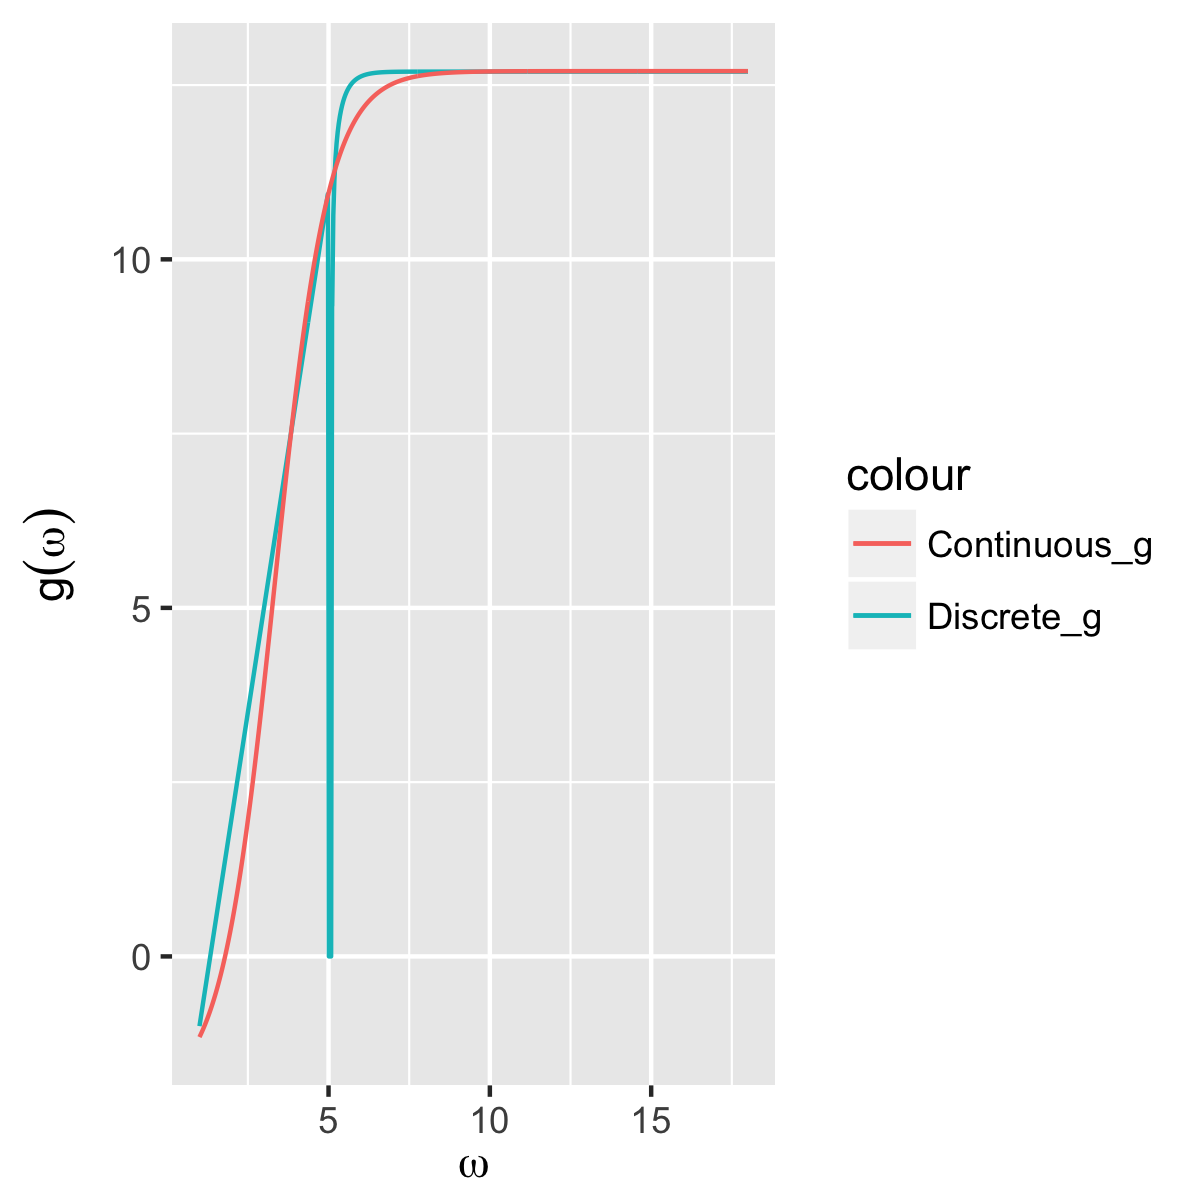
\includegraphics{plot_g}
  \caption{Plot of both versions of $g(\omega)$}
  \label{plot_g}
\end{figure}

The single period objective function for firm 1 as a function of the industry state, $S$, the actions of firm 1, $\mu_1$, and the other firms' actions, $\mu_2$, can be expressed with the following equation. Let $\mu_j=\{p_j,x_j\}$, where $p_j$ represents the price charged to consumers for product j and $x_j$ represents the level that firm j invests into the quality of their product. $M$ represents the market size, and $c$ represents the marginal cost of production. The single period payoff function is

\begin{equation*}
  \pi_1(S,\mu_{1},\mu_{2})=M \frac{\text{exp}(g(S_1)-p_1)}{1+\text{exp}(g(S_1)-p_1)+\text{exp}(g(S_2)-p_2)} (p_1-c)-x_1
\end{equation*}

In order to calculate the expected future value for a policy $\mu_1$ let

\begin{equation*}
  \mathbb{E}[\hat{V}(S'|S,\mu_{1},\mu_{2})] = \sum_{\omega'_1=1}^m \sum_{\omega'_2=1}^m \hat{V}(\{\omega'_1,\omega'_2\}) \text{Pr}(\omega'_1|\omega_1,x_{1}) \text{Pr}(\omega'_2|\omega_2,x_{2})
\end{equation*}

Where the probability of transitioning to the state $\omega'$ given investment $x$ and current state $\omega$ is given by

\begin{equation*}
  \text{Pr}(\omega'|\omega,x) =
  \begin{cases}
    \frac{(1-\delta) \alpha x}{1+\alpha x} & \text{if } \omega'=\omega+1\\
    \frac{1-\delta+\delta \alpha x}{1+\alpha x} & \text{if } \omega' = \omega\\
    \frac{\delta}{1+\alpha x} & \text{if } \omega' = \omega-1\\
  \end{cases}
\end{equation*}

\begin{equation*}
  \text{Pr}(\omega'|1,x) =
  \begin{cases}
    \frac{(1-\delta) \alpha x}{1+\alpha x} & \text{if } \omega'=2\\
    \frac{1+\delta \alpha x}{1+\alpha x} & \text{if } \omega'=1\\
  \end{cases}
\end{equation*}

\begin{equation*}
  \text{Pr}(\omega'|L,x) =
  \begin{cases}
    \frac{1-\delta+\alpha x}{1+\alpha x} & \text{if } \omega'=L\\
    \frac{\delta}{1+\alpha x} & \text{if } \omega'=L-1
  \end{cases}
\end{equation*}

where $\delta$ represents the probability that the outside alternative increases in quality, and $\alpha$ represents the efficacy of investment in generating increases in efficiency. Through out the paper I will reference the MPE of this model found when $\beta=0.925$, $M=5$, $c=5$, $\alpha=3$, and $\delta=0.7$.

\subsection{Pakes-McGuire algorithm}

% Like all backward solution techniques the Pakes and McGuire (1994) algorithm is an iterative procedure which starts each iteration with a set of numbers in memory, provides a rule which updates those numbers in the course of the iteration, and checks to see if the updated numbers satisfy a convergence criterion at the end of the iteration. If not the algorithm begins a new iteration.
% 2007_Doraszelski_Pakes

The \citet{1992_Pakes_McGuire_NBER} algorithm is an iterative backward solution method which uses numbers stored in memory from the previous iteration to calculate an update to those numbers and runs until the updated numbers satisfy a convergence condition. At the start of the algorithm $N$ approximation nodes, $\{S_i\}_{i=1}^N$, must be chosen. Each node represents a possible industry state that can be visited in the model. It is also necessary to initialize an $\epsilon>0$ for the convergence criterion and to initialize the value function.
% If the value function is initialized at $0$ then the backward solution method can be interpreted as the limit of a finite stage game where the final period is valued at $0$. (maybe not for pakes mcguire)

The algorithm uses the assumption that firms use symmetric strategies so that only one value function needs to be calculated. For notational purposes I will denote the firm for which the value function is calculated as firm 1. Since we are interested in finding only symmetric MPE, the \citet{1992_Pakes_McGuire_NBER} algorithm uses the calculation of firm 1's policies in iteration k-1 to determine the policies of all other firms in iteration k. For example, in the numerical example the pricing policy for firm 2 in state $S_i$, and iteration k is represented as $p^{k}_{i,2}=p^{k-1}_{i',1}$ where $i'$ is such that if $S_i=\{\omega_1,\omega_2\}$ then $S_{i'}=\{\omega_2,\omega_1\}$.

More generally, for each iteration $k$ the algorithm uses firm 1's policy from last iteration, $\mu^{k-1}_1$ to determine the policy that other firms will choose, $\mu^k_{-1}$, and then calculates $\mu^k_1$ based on $\mu^k_{-1}$ and $v_i^{k-1}$. Then the algorithm checks a convergence condition by evaluating the distance between the previous iterations value function and the current value function.

\begin{algorithm}[H]
  \caption{Pakes McGuire Algo}
  \begin{algorithmic}[1]
    \Procedure{}{} Choose $N$ approximation nodes $\{S_i\}_{i=1}^N$, error tolerance for value function updating $\epsilon$.
    \State Let $v^0_i=0$ for $i=1,\dots,N$
    \While{$\norm{v^{k}_1-v^{k-1}_1} > \frac{\epsilon (1-\beta)}{2\beta}$}
    \For{$i=1,\dots,N$}
    \State Solve the Bellmann equation and store in memory $v^k_{i,1}$ and $\mu^k_{i,1}$
    \begin{equation*}
      v^k_{i,1}=\max_{\mu^k_{i,1} \in \Gamma(S_i)} \pi(S_i, \mu^k_{i,1}, \mu^{k-1}_{i,-1})+ \beta\mathbb{E}[\hat{V}(S')|S_i,\mu^k_{i,1},\mu^{k-1}_{i,-1})]
    \end{equation*}
    \State Let $k=k+1$
    \EndFor
    \EndWhile
    \EndProcedure
  \end{algorithmic}
\end{algorithm}

The run time of this algorithm can be approximated with the following formula. Let K represent the number of value function iterations required for convergence, N the number of states in the state space, and $f_{evals}$ be the number of function evaluations required to find the optimal policy.

\begin{equation}
  \label{runtime}
  \begin{split}
  \text{run time} &= (K)(N)(f_{evals})(\text{Computation time of f})\\
  H(S_i)&=\max_{\mu^k_{i,1} \in \Gamma(S_i)}f(S_i,\mu^k_{i,1})\\
  f(S_i,\mu^k_{i,1})&=\pi(S_i, \mu^k_{i,1}, \mu^{k-1}_{i,-1})+ \beta\mathbb{E}[\hat{V}(S')|S_i,\mu^k_{i,1},\mu^{k-1}_{i,-1})]
  \end{split}
\end{equation}

This algorithm suffers from several computational issues. There are curses of dimensionality in both the state space and action space that can cause the algorithm to take too long to run. For a fixed number of iterations required for convergence, which I will denote as $K$, if the industry of interest has just 10 firms then $N$ can be too large. In the numerical example in this paper, each firm has 18 possible states and so for 10 firms, the size of the state space would be $18^{10}=3,570,467,226,624=N$. If the time it takes to compute $f(S,\mu)$ takes just 0.01 seconds then it would take 413,248 days to just evaluate the function once in each state. There are many different ways to decrease the computational cost imposed by increasing the number of firms, and in \hyperref[state]{Section \ref{state}} I will show several methods of value function approximation to overcome this issue.

In applications of the \citet{1995_Erickson_Pakes_RES} framework firms can have many decision variables. Typically a firm chooses the price of their product, how much to invest to improve their state, and whether to enter or exit, however many firms can have a much more complex decision making process. In the numerical example used in this paper firms just choose the price of their product and level of investment to improve the quality of their product. In order to choose the optimal action using a simple grid search procedure with a 1e-5 degree of accuracy there would need to be a 400,000 by 500,000 grid representing each possible choice that the firm could make (since in equilibrium the optimal price varies from 6 to 11 and the optimal level of investment varies from 0 to 4). Thus, the number of function evaluations per state per iteration, which I will denote as $f_{evals}$, would be 200,000,000,000. An algorithm implemented this way would take 23,148 days to find the optimal action in a single state in a single iteration. There are many different methods that allow the optimal action to be found with a high degree of accuracy very quickly and \hyperref[action]{Section \ref{action}} discusses how to use these methods to decrease $f_{evals}$.

In many applications the run time required to compute an equilibrium determines the way in which the theoretical model was written \citep{2007_Doraszelski_Pakes, 2015_Benkard_Weintraub_Jeziorski_RAND}. Often, this leads to including only 2-4 firms, or using a profit function that can be computed outside the algorithm's main loop to reduce the number of decision variables.

Thus in order to develop richer models of industry dynamics that are a closer representation of reality, it is important to understand the factors that determine a models run time and the methods that can be used to make a model computationally tractable.

\section{Avoiding the curse of dimensionality in action space}
\label{action}

In order to reduce the computational cost caused by a curse of dimensionality in the action space it is necessary to either reduce the number of decision variables, or reduce the number of function evaluations required to find the policy that maximizes the objective. In the \citet{1995_Erickson_Pakes_RES} framework it is common to use a static-dynamic breakdown to reduce the number of decision variables. A static-dynamic breakdown means that the model is constructed in such a way that in the dynamic industry it is optimal for firms to choose the same prices that they would choose in a single period model. If this is the case then the profitability for firm 1 in each state only has to be computed once and then stored in memory. In some settings it is not desirable to use a static-dynamic breakdown since the pricing decision does influence the dynamics of the industry. This is the case in dynamic network industries where the price of a product in a period t affects the market share for each firm in t+1 \citep{2009_Chen_Doraszelski_Harrington, 2006_Mitchell_Skrzypacz, 2006_Chen_Doraszelski}.

If there several decision variables, a high degree of accuracy is required, or the run time is too large it is advantageous to use more sophisticated methods to find the optimal policy in a state. The first issue that arises is if the decision variable is continuous. Exit and entry decisions are naturally modeled as a discrete 0 for exit and 1 for remaining in the industry, but many other policy decisions, such as how much to invest, or the price charged for a product are most naturally modeled as a continuous variable. Since in the \citet{1995_Erickson_Pakes_RES} framework the state space is discretized in order for $H(S)$ to be well defined it is necessary to map continuous actions to discrete future states. This is because the objective function $f(S,\mu)$ contains the evaluation of the expected value of future payoffs conditional on the current state and actions. In this expectation the value function $V : S' \in \{S_i^N\} \rightarrow \mathbb{R}$ can only be evaluated if $S' \in \{S_i^N\}$ where $S'=h(S,\mu)$. The transition function $h(S,\mu)$ maps the policy $\mu$ and discrete states $S$ to discrete states $S'$. In the numerical example used in this paper the transition function represents the change in quality a firm receives as a function of their current quality and level of investment. The transition function is restricted to increasing quality by one level, remaining at the current level, or decreasing quality by one level and the probability of each event is conditional on the level of investment, $x$.

In order to discuss numerical optimization methods for it is helpful to rewrite the right hand side of the Bellman equation as

\begin{equation}
  \label{hdef}
  \begin{aligned}
    & H(S)=\max_{\mu} f(S,\mu) \\
    \text{s.t.}\quad & g(S, \mu)=0,\\
    & h(S,\mu) \geq 0
  \end{aligned}
\end{equation}

The most straight forward approach to solving this problem is to use a simple grid search. To do the grid search you choose a grid for each element in the vector $\mu$ and then evaluate $f$ at each point in the grid and then choose the action that has the largest value. While this method will find the global maximum of $f$ up to the accuracy limit imposed by how fine the grid is, this method requires far too many function evaluations to be used in many contexts.

The numerical analysis literature has produced many algorithms that have far better convergence rates to the optimal action and there are many efficiently implemented software packages that makes using these algorithms very easy. However, the run time required to find the optimal action varies significantly based on which method was chosen, the problem's structure, and the specific way that the algorithm was implemented in a software package.

The first numerical optimization algorithm I used for solving this problem was the method presented in \citet{ipopt} and implemented in the C++ library IPOPT. This method is a derivative free algorithm for solving constrained optimization problems and is also one of the most standard computational methods for solving non-linear optimization problems with constraints. It is also the default method for MATLAB's function fmincon. When I used this algorithm for the numerical example, it had convergence issues and the software implementation was not suited to dynamic programming applications. This is because dynamic programming applications require the numerical method to be applied inside a for loop for the value function iterations and inside a for loop that is iterating over each approximation node. This means that the algorithm and software implementation should have limited overhead and not require access to a solver outside of the source code which the IPOPT library did.

Due to these limitations I then used the C++ library NLOPT since it does not have the implementation issues that IPOPT has \citep{nlopt}. This library provides access to many different optimization methods. The numerical methods to solve constrained non-linear optimization problems can be categorized into several categories. The first category, global optimization focuses on finding the global maximum. For example, the DIRECT algorithm presented in \cite{direct} relies on the systematic division of the search domain into smaller and smaller hyperrectangles. Methods in this category are typically very slow and thus are not tractable for the applications of interest.

The second category is local derivative-free optimization algorithms. I compared NLOPT's implementation of the Constrained Optimization by Linear Approximations (COBYLA) presented in \citep{cobyla1, cobyla2} to IPOPT's method. While methods in this category are not guaranteed to find the global optimum they are much faster and perform well on convex problems. I found that COBYLA was able to converge however the method required approximately 50 function evaluations per state per value function iteration to find the optimal action within a tolerance of 1e-5.

The third category is local gradient-based optimization algorithms. These methods require the analytical gradient of the optimization problem with respect to the decision variables to be supplied. This gradient is often easy to analytically derive and supply to the algorithm in the applications of interest. These methods have been shown to converge at a much faster rate than derivative-free algorithms \citep{friendly}. I compared the L-BFGS algorithm presented in \citep{bfgs1, bfgs2} with the COBYLA method and found that L-BFGS required approximately 5.6 function evaluations per state per value function iteration to find the optimal action within a tolerance of 1e-5. Local gradient-based optimization algorithms also do not suffer from the curse of dimensionality in the action space which makes them attractive for applications where there are hundreds of decision variables and many constraints. This advancement in numerical analysis allows economic researchers to model firms with  more realistic and complicated action spaces.

These methods all improve upon the simple grid search algorithm and depending on the context dramatically reduce $f_{evals}$. The derivative free methods however will still suffer from the curse of dimensionality in the action space that occurs when there are many decision variables. In order to overcome this issue it is recommended to analytically supply the gradient of $f$ with respect to $\mu$ to the algorithm. If you supply the analytical gradient then it is possible to use algorithms in the local gradient-based optimization category which have been shown to further reduce $f_{evals}$ and also overcome the curse of dimensionality in the action space.

\section{Avoiding the curse of dimensionality in state space}
\label{state}
% The convergence problems were likely to result from the fact that in their model the firm’s value function can be a discontinuous function of its competitor’s policies (entry and exit by competitors can cause jumps in the value function), and the polynomials they used have problems approximating discontinuities. So these problems may well disappear if either different forms of approximations were used (e.g. splines), or if the number of firms grew larger (in which case exit by any one firm should have a smaller effect on the value of its competitors). This suggests that function approximation might still be a useful technique for problems with a large number of firms (as is often the case in the dynamic models used in trade, development, and productivity), though such applications might require some further technical developments.
% 2007_Doraszelski_Pakes

The curse of dimensionality in the state space is often a more difficult issue to overcome. Typically, it is easier to solve computationally a model that is discrete rather than a continuous one and when the dimension of the state space is small and this is true in the \citet{1995_Erickson_Pakes_RES} framework. However when the state space is large it is computationally more efficient to approximate the discrete state space with continuous functions.

There are many different methods for approximating a function evaluated at a few discrete points in one dimension. For example, if I was interested in approximating the function $v(S)=\text{sin}(S)$ where $S \in [0, 4\pi]$. If I had the Lagrange data, $\{S_i,v_i\}_{i=1}^N$, where $S_i=\frac{4\pi i}{N}$, $v_i=\text{sin}(S_i)$, and $N=6$ then I could use many different interpolation methods. One method that I could used called polynomial interpolation with Chebyshev polynomials uses a sum of orthogonal polynomials to approximate the function $v$.

Chebyshev polynomials can be defined using a recursive definition or using a trionmetric definitive. Using the trigonometric definition, a $n$ degree Chebyshev polynomial of the first kind is defined as

\begin{equation*}
  T_n(S)=\text{cos}(n \text{ arcos}(\frac{2S-S_{min}-S_{max}}{S_{min}-S_{max}}))
\end{equation*}

If $S_{min}=-1$ and $S_{max}=1$ then the first four polynomials will be

\begin{equation*}
  \begin{aligned}
    T_0(S)&=1\\
    T_1(S)&=S\\
    T_2(S)&=2S^2-1\\
    T_3(S)&=4S^3-3S\\
    T_4(S)&=8S^4-8S^2+1
  \end{aligned}
\end{equation*}


\begin{figure}[H]
  \label{plot_cheb_4}
  \centering
  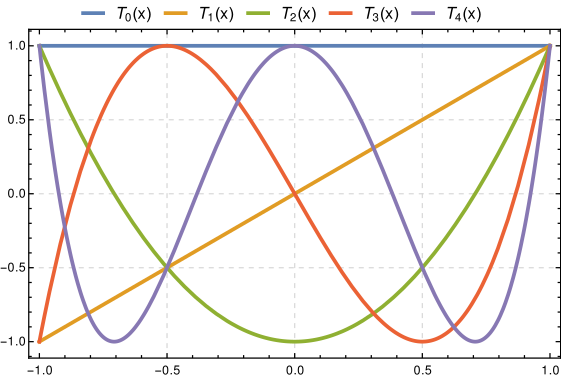
\includegraphics[scale=3]{plot_Chebyshev_Polynomials_of_the_First_Kind}
  \caption{The first four Chebyshev polynomials}
\end{figure}

and then approximation can be written as $\hat{V}(S;b)=\sum_{k=0}^n b_k T_k(S)$.
When interpolating a function with Chebyshev polynomials it is important to choose the approximation nodes based off of the roots of the polynomials. The Chebyshev nodes for one dimension are given by $S_i=(z_i+1)(S_{max}-S_{min})/2+S_{min}$ and $z_i=-\text{cos}((2i-1)\pi/(2m))$ where $m$ is the number of approximation nodes. In order to approximate the function $v(S)$ using the Lagrange data $\{S_i,v_i\}_{i=1}^N$, where $v_i=v(S_i)$, it is necessary to solve for the coefficients, $b$, using

\begin{equation*}
  \min_{\boldsymbol{b}}\sum_{i=1}^N (\hat{V}(S_i;\boldsymbol{b})-v_i)^2
\end{equation*}

This problem can be solved easily with OLS or with the Chebyshev Approximation Formula. This approximation method has a few cases where it performs poorly. One case where the approximation is poor is when $N$ is too small. For a fixed $N$ the approximation can be improved by fittiting the polynomial approximation using Hermite data. Hermite data consists of the approximation node, the function evaluated at the approximation node and also the gradient of the function evaluated at the approximation node. In order to fit the Chebyshev polynomial using Hermite data, $\{S_i,v_i,d_i\}_{i=1}^N$, where $d_i=\frac{d v(S_i)}{d S}$, the coefficients are found by solving the following OLS problem.

\begin{equation*}
  \min_{\boldsymbol{b}} \sum_{i=1}^N\bigg((\hat{V}(S_i;\boldsymbol{b})-v_i)^2 + (\frac{\partial \hat{V}(S_i;\boldsymbol{b})}{\partial S} - d_i)^2 \bigg)
\end{equation*}

Chebyshev polynomials are an attractive choice for fitting a function using Hermite data since the derivative of type 1 Chebyshev polynomials are a function of type 2 Chebyshev polynomials. Since $\frac{\partial T_n(S)}{\partial S} = n U_{n-1}(S)$ and type 2 Chebyshev polynomials can be defined by the following equation.

\begin{equation*}
  U_n(S) = \frac{\text{sin}((n+1) \text{arccos}(\frac{2S-S_{min}-S_{max}}{S_{min}-S_{max}}))}{\text{sin}(\text{arccos}(\frac{2S-S_{min}-S_{max}}{S_{min}-S_{max}}))}
\end{equation*}

By incorporating the gradient information a function can be approximated to a given degree of accuracy with fewer approximation nodes. \hyperref[ref_Cheb_Sin_Func]{Figure 3} shows how Hermite approximation is able to approximate the function $\text{sin}(x)$ with four approximation nodes to a much better degree of accuracy than the Lagrange approximation.

\begin{figure}[H]
  \centering
  \label{ref_Cheb_Sin_Func}
  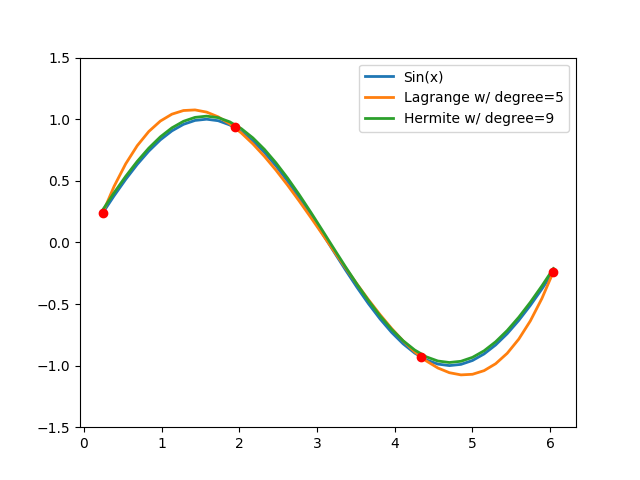
\includegraphics[scale=.8]{plot_Cheb_Sin_Func}
  \caption{Lagrange and Hermite Chebyshev approximation of Sin(x)}
\end{figure}

Another case where polynomial approximations perform poorly is when there are large discontinuities or non-linearities in the function that is being approximated. When trying to approximate a discontinuous function polynomial approximations can often show the Gibbs phenomenon which is when the approximating polynomial overshooting or undershooting the function around a jump discontinuity. This overshooting/undershooting persists even when the number of approximation nodes increases. This can be seen in \hyperref[ref_Cheb_Ind_Func]{Figure 4} when Lagrange and Hermite Chebyshev polynomials are used to approximate the function $f(x)$ with 10 approximation nodes.

\begin{equation}
  \label{ind_func}
  f(x)=\begin{cases}
    1 & \text{ if } x\leq1/2\\
    0 & \text{otherwise}
  \end{cases}
\end{equation}

\begin{figure}[H]
  \label{ref_Cheb_Ind_Func}
  \centering
  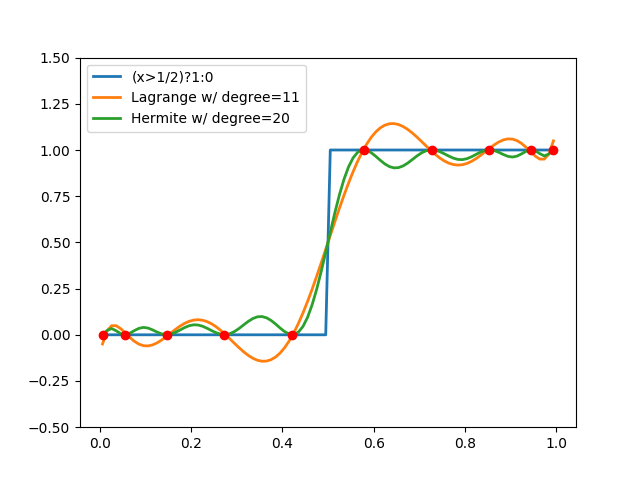
\includegraphics[scale=.8]{plot_Cheb_Ind_Func}
  \caption{Lagrange and Hermite Chebyshev approximation of f(x)}
\end{figure}

In order to overcome this issue it is necessary to use an approximation techinque that is able to approximate the function locally. This can be done by fitting a piecewise linear function however, piece-wise linear functions are not smooth and the kink that occurs at each approximation node can cause problem when used for value function approximation. Cubic splines are smooth and can approximate the function locally however this method does not generalize to n dimensions.

\cite{ann_uni} show that Artificial Neural Nets are universal approximators. Artificial Neural Nets are able to approximate functions locally to avoid the Gibbs Phenomenon, and also scale very easily to approximating multidimensional functions. There has also been a large influx of computationally efficient software packages for training and evaluating neural nets. For an introduction to ANN please refer to \citet{ann_tutorial}.

\begin{figure}[H]
  \label{ref_ANN_Ind_Func}
  \centering
  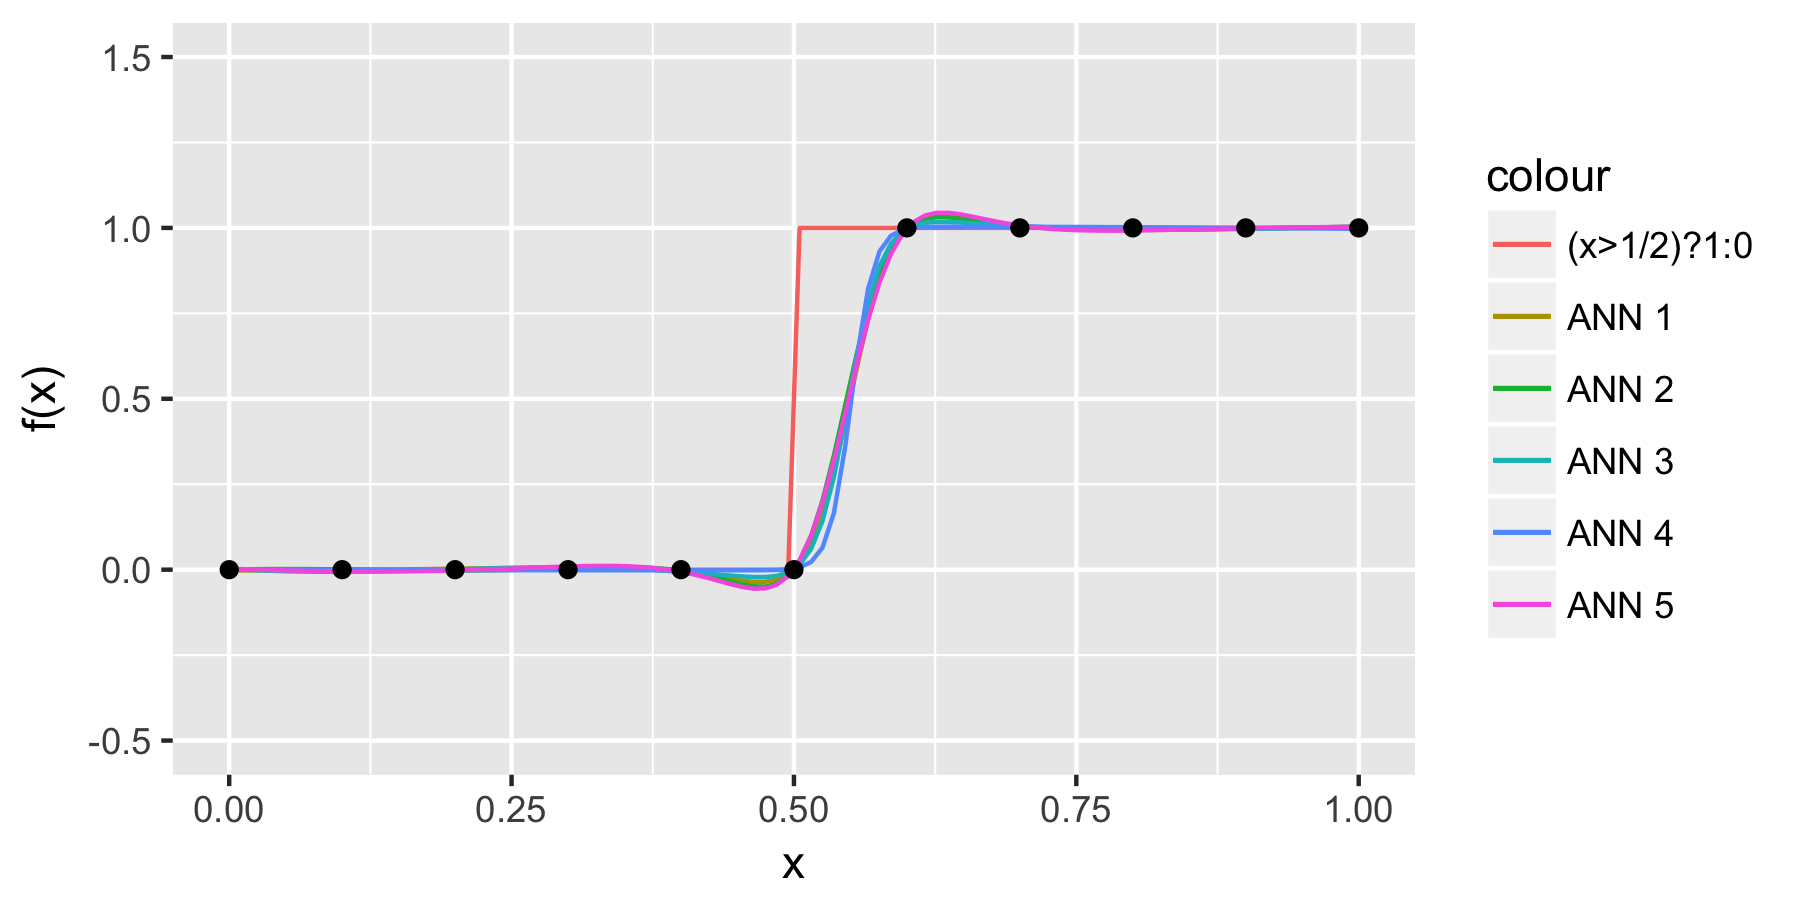
\includegraphics[scale=1]{plot_ANN_Ind_Func}
  \caption{ANN approximation of f(x)}
\end{figure}

\hyperref[ref_ANN_Ind_Func]{Figure 5} shows how a ANN with a single hidden layer with 10 nodes was able to approximate the function without the same issues that Chebyshev polynomials had. The graph was created using the same ANN but trained 5 times and each time starting out with a different set of random initial parameters. This figure also shows a drawback of using ANN, which is that they sometimes get stuck in local minimum. This can be seen with the fifth approximation. \citet{ann_radial} showed that using different network structures such as a Radial Basis Function Network or a Wavelet Neural Network can improve the accuracy of ANN by reducing the frequency that the ANN gets stuck in a local minimum. \citet{ann_disc} show that ANN can approximate any discontinuous function with a single hidden layer and \citet{ann_herm} also show that the Hermite approximation problem can be solved using ANN.

Using either Chebyshev polynomials or ANN to approximate a function allows for an accurate representation of a continuous function using a relatively small set of points. In the following algorithm these techniques will be used to approximate the value function of firm 1. By approximating the value function, it is possible to reduce the number of approximation nodes required to solve for an equilibrium.

\begin{algorithm}[H]
  \caption{Pakes McGuire Algo with L-VFA}
  \begin{algorithmic}[1]
    \Procedure{}{} Choose $N$ approximation nodes $\{S_i\}_{i=1}^N$, error tolerance for value function updating $\epsilon$.
    \State Initialize $\boldsymbol{b}$
    \While{$\norm{\hat{V}^{k}_1-\hat{V}^{k-1}_1} > \frac{\epsilon (1-\beta)}{2\beta}$}
    \For{$i=1,\dots,N$}
    \State Solve the Bellmann equation and store in memory $\hat{V}^k_{i,1}$ and $\mu^k_{i,1}$
    \begin{equation*}
      v^k_{i,1}=\max_{\mu^k_{i,1} \in \Gamma(S_i)} \pi(S_i, \mu^k_{i,1}, \mu^{k-1}_{i,-1})+ \beta\mathbb{E}[\hat{V}(S';b)|S_i,\mu^k_{i,1},\mu^{k-1}_{i,-1})]
    \end{equation*}
    \State Minimize the mean squared error and store in memory $\boldsymbol{b}$
    \begin{equation*}
      \min_{\boldsymbol{b} \in \Omega} \sum_{i=1}^N \bigg ( v^k_{i,1} - \hat{V}(S_i;\boldsymbol{b}) \bigg)^2
    \end{equation*}
    \State Let $k=k+1$
    \EndFor
    \EndWhile
    \EndProcedure
  \end{algorithmic}
\end{algorithm}

This algorithm replaces the discretized value function with a continuous approximation. Since the value function can now be approximated by a continuous and differentiable function it is now possible to solve for an equilibrium of a model that uses a continuous state space. This is attractive feature since empirically the return from investment is continuously distributed, and since firms do not have a set of predetermined discrete levels of quality and so VFA allows for a more realistic theoretical model in addition to a more computationally efficient method for solving for an equilibrium.

Using the numerical example in this paper I compared the equilibrium found using two methods on six different grids of approximation nodes. The first method was using multidimensional Chebyshev polynomials to approximate the value function and the second method was a ANN with a single layer. When using the Chebyshev polynomials I used a grid based on the location Chebyshev nodes which are defined by $x_i=(z_i+1)(x_{max}-x_{min})/2+x_{min}$ and $z_i=-\text{cos}((2i-1)\pi/(2m))$ where $m$ is the number of approximation nodes per firm. When using the ANN I used an equidistant gird of $m$ points per firm. I examined the equilibrium value function and policy functions found when $m=6,12,\text{and }18$.

The results show that the ANN was able to approximate the value function to a high enough degree of accuracy that the equilibrium policy functions maintained their qualitative structure when $m=6,12,\text{and }18$. The multidimensional Chebyshev approximation was able to preserve the policy function's qualitative structure when $m=12, \text{and } 18$ however, when $m=6$ the value function failed to converge. The approximation failed to converge because when the value function increases very quickly when firm 2's state is at a low value of about 3 and firm 1's state is between 3 and 6. This large rate of increase leads the approximation to exhibit the Gibbs Phenomenon which can be seen in \hyperref[gibbslittle]{Figure \ref{gibbslittle}} and more prominently in  \hyperref[gibbsmore]{Figure \ref{gibbsmore}} \footnote{\href{https://github.com/wmjones/VFA-for-dynamic-games}{My Github Repository} has the source code, an easy to use makefile, and animated gifs of each of the 6 examples where each frame of the gif is a value function iteration.}. This is especially an issue because during the value function iterations the region that was overshot is reinforced and the approximation error propagates through the subsequent value function iterations.

These results suggest that ANN are able to approximate the value function to a higher degree of accuracy than Chebyshev polynomials when the number of approximation nodes is reduced. This is useful since if Chebyshev polynomials can approximate it with a sufficient degree of accuracy when $m=12$ and ANN can approximate the value function with a sufficient degree of accuracy when $m=6$, then with 10 firms VFA with Chebyshev polynomials is approximately 60 times faster than a method that uses $m=18$ and VFA with ANN is approximately 60,000 times faster than a method that uses $m=18$.

L-VFA can also be easily combined with other methods for reducing the size of the state space. For example, it is easy to use parallelization to reduce the computational cost of the algorithm by finding the value of each state in parallel. This approximately divides the run time of the algorithm by the number of threads that evaluation of each state is parallelized over. In the numerical example I parallelized over 8 threads to reduce computation time.

It is also easy to incorporate other methods to reduce the size of the state space. \citet{1992_Pakes_McGuire_NBER} show that
\begin{equation*}
  V(\omega_1,\omega_2,\dots,\omega_N)=V(\omega_1,\omega_{\pi(2)},\dots,\omega_{\pi(n)})
\end{equation*}
for any $n-1$ dimensional vector $\pi=[\pi(2),\dots,\pi(n)]$ which is a permutation of $(2,\dots,n)$. Therefore, the value function does not need to be evaluated at each distinct approximation node but instead only needs to be evaluated at the nodes where $\omega_2\geq \omega_3,\dots,\geq \omega_n$. This causes the number of approximation nodes in the state space to be calculated as $\frac{(m+n-1)!}{(m-1)!n!}$ instead of $m^n$. For 10 firms and $m=18$ this leads to $N=8,436,285$, when $m=12$ this leads to $N=352,716$ and when $m=6$ this leads to $N=3,003$. Thus if it takes approximately 0.01 seconds to evaluate the function $f$, it will now only take 23.4 hours to do one value function iteration when $m=18$, 0.98 hours to do one value function iteration when $m=12$ and only 0.008 hours to do one value function iteration when $m=6$. This reduction in computation time allows for the exploration of richer models with larger state spaces which were previously unable to be analyzed due to computational constraints.

Similar to how the approximation accuracy of one dimensional functions can be improved by fitting Hermite data rather than Lagrange data, the value function can be approximated using Hermite data. \citet{2015_Judd_Cai} discuss a method for easily obtaining the gradient of the value function in order use Hermite data to approximate the value function. \citet{2015_Judd_Cai} showed that Hermite value function approximation (H-VFA), was able to either produce a higher accuracy in a given amount of time or attain the same accuracy with much less computation time when compared to L-VFA.

If the right hand side of the Bellman equation is written as

\begin{equation}
  \begin{aligned}
    & H(S)=\max_{\mu} f(S,\mu) \\
    \text{s.t.}\quad & g(S, \mu)=0,\\
    & h(S,\mu) \geq 0
  \end{aligned}
  \label{equationA}
\end{equation}

then the gradient of $H(S)$ is provided by

\begin{equation*}
  \frac{\partial H(S)}{\partial S_j} =\frac{\partial f}{\partial S_j}(S, \mu^*(x)) + \lambda_1^*(S)^T\frac{\partial g}{\partial S_j}(S, \mu^*(S)) + \lambda_2^*(S)^T\frac{\partial h}{\partial S_j}(S, \mu^*(S))
\end{equation*}

For $j=1,\dots,n$ and $n$ is the dimension of $S$. The computation of the gradient requires finding several derivatives and is difficult to compute. However, the problem can be rewritten by adding in the variable $y$ such that

\begin{equation}
  \begin{aligned}
    & H(S)=\max_{\mu,y} f(y,\mu) \\
    \text{s.t.}\quad & g(y, \mu)=0,\\
    & h(y,\mu) \geq 0,\\
    & S_j-y_j=0,\quad j=1,\dots,n.
  \end{aligned}
  \label{equationB}
\end{equation}

Then the gradient of $H(S)$ is provided by

\begin{equation*}
  \frac{\partial H(S)}{\partial S_j} = \tau^*_j(S)
\end{equation*}
where $\tau^*_j(S)$ is the Lagrange multiplier for the constraints $S_j-y_j=0$.

There are several derivative-free constrained optimization software libraries that provide along with the solution to the maximization problem the Lagrange multiplier for each constraint. This method allows for an easy method to obtain the gradient of the value function and thus able to use the Hermite data, $\{S_i,v_i,d_i\}_{i=1}^N$, where $d_i$ is the gradient vector evaluated at $S_i$, to approximate the value function.

The coefficients to approximate the value function using multidimensional Chebyshev polynomials are obtained by solving the following equation and the notation for multidimensional Chebyshev polynomials is presented in \hyperref[multicheb]{Appendix 2}.

\begin{equation*}
  \min_b \Bigg \{\sum_{i=1}^N \bigg (v_i-\sum_{0\leq |\alpha|\leq r}b_\alpha T_\alpha(S_i) \bigg )^2+\sum_{i=1}^N \sum_{j=1}^{n} \bigg ( d_{i,j} - \sum_{0\leq |\alpha|\leq r}b_\alpha \frac{\partial}{\partial S_j}T_\alpha(S_i) \bigg )^2 \Bigg \}
\end{equation*}

While the L-VFA algorithm presented in \citet{2015_Judd_Cai} is easily added to the Pakes McGuire Algorithm, the H-VFA algorithm is not directly applicable. A direct adaptation of H-VFI for the Pakes McGuire Algorithm would be

\begin{algorithm}[H]
  \caption{Pakes McGuire Algo with H-VFA using Chebyshev Polynomials}
  \begin{algorithmic}[1]
    \Procedure{}{} Choose $N$ approximation nodes $\{S_i\}_{i=1}^N$, error tolerance for value function updating $\epsilon$.
    \State Initialize $\boldsymbol{b}$
    \While{$\norm{\hat{V}^{k}_1-\hat{V}^{k-1}_1} > \frac{\epsilon (1-\beta)}{2\beta}$}
    \For{$i=1,\dots,N$}
    \State Obtain the value function at $S_i$, and gradient by solving Equation \eqref{equationA} or Equation \eqref{equationB}. Then store in memory $v^k_{i,1}$, $\mu^k_{i,1}$, and $d_{i}^k$.
    \State Minimize the mean squared error and store in memory $b$ using Hermite data $\{S_i,v_{i,1},d_{i,1}\}_{i=1}^N$ by solving
\begin{equation*}
  \min_{\boldsymbol{b}} \Bigg \{\sum_{i=1}^N \bigg (v_i-\sum_{0\leq |\alpha|\leq r}\boldsymbol{b}_\alpha T_\alpha(S_i) \bigg )^2+\sum_{i=1}^N \sum_{j=1}^{n} \bigg ( d_{i,j} - \sum_{0\leq |\alpha|\leq r}\boldsymbol{b}_\alpha \frac{\partial}{\partial S_j}T_\alpha(S_i) \bigg )^2 \Bigg \}
\end{equation*}
    \State Let $k=k+1$
    \EndFor
    \EndWhile
    \EndProcedure
  \end{algorithmic}
\end{algorithm}

Step 5: in this algorithm causes complications. Since the reaction of other firms is taken into account a firm's decision the gradient calculation using \eqref{equationA} would require the calculation of the gradient of the policy function. This is because the policy that the other firms choose depends on what the industry's state is. Thus in order complete Step 5: using Equation \eqref{equationA} it is necessary to determine the gradient of the policy function. Since the analytical gradient of the policy function cannot be obtained it is necessary to numerically approximate the gradient. This can be done easily with the central difference method. The accuracy of the central difference method is limited by the step size which in this context is the distance between two approximation nodes. Thus in order to obtain an accurate approximation of the policy function there would need to be more approximation nodes which prevents H-VFA from decreasing the number of approximation nodes.

If Step 5: is calculated using \eqref{equationB} then there can be an issue with the numerical optimization method converging. This is due to the fact that a derivative free algorithm is used to calculate the solution and that by adding in an additional decision variable $y$ the number of function evaluations required to find the optimal action will grow significantly. Therefore the computational cost of finding the optimal action may cause the Pakes Mcguire Algorithm with H-VFA to be slower than Pakes Mcguire Algorithm with L-VFA.

% section 5 prop 3 of 1994_Pakes_McGuire show that approx with symmetry leads to constant state space size

% \section{Approximation as a Behavioral Model}

\section{Conclusion}
\label{con}

I have shown how to incorporate numerical optimization methods to avoid the curse of dimensionality in the action space and that by adding value function approximation to the Pakes McGuire algorithm it is possible to reduce the number of states needed per firm. I have also discussed the benefits that ANN have over multidimensional Chebyshev polynomials for value function approximation and the complications that arise from attempting to fit the value function using Hermite data in dynamic game models. These conclusions are supported by a numerical example of the Pakes McGuire quality ladder model.

The L-VFA numerical example when fit with ANN used a simple single hidden layer ANN. Future research could examine the benefits to using more complex network structure such as deep neural networks. \citet{anndeep} show that the number of neurons needed to approximate a function decreases exponentially in the number of layers in the network. Future research could also incorporate other methods from approximate dynamic programming such as using post-decision state sampling to reduce the computational cost of computing the expected value, or using ANN to construct a continuous implementation of the dynamic lookup table presented in \cite{dlt}.

% It should be clear from the discussion above that the burden of computing equilibria can often be a significant consideration in choosing the model we analyze. Indeed we typically can add enough sources of heterogeneity to any applied problem to make it impossible to compute the required equilibrium.19 Moreover this same caveat will apply to the more sophisticated algorithms introduced below. On the other hand, all applied work can ever hope to accomplish is to form an approximation to the work- ings of real industries that is adequate for the problem being analyzed. What the more sophisticated algorithms allow us to do is weaken the dominance of computational con- siderations in considering the relevant tradeoffs.
% 2007_Doraszelski_Pakes

\bibliographystyle{apacite}
\bibliography{bibliography.bib}

\section*{Appendix 1: Plots}

In each plot the top row is the value function, the middle row is the policy function for investment, and the bottom row is the policy function for product price. Each column shows a different view of the 3D graph where the first column shows firm 2's quality increasing on the left and firm 1's quality increasing on the right. The middle column shows a rotation of the first column so that firm 1's quality is increasing to the right and the right column the rotation such that firm 1's quality is decreasing to the right. The top row was generated by evaluating the value function approximation on a grid of 150x150 points, and coloring the points based on their value. The middle and bottom rows cannot be evaluated in this way since the algorithm presented do not interpolate the policy functions. Since it is hard to see the structure of the policy functions when only examining discrete points I interpolated the policy functions using a Delaunay triangulation method from the package deldir in R \citep{deldir}.

\begin{figure}[H]
  \centering
  \makebox[\textwidth]{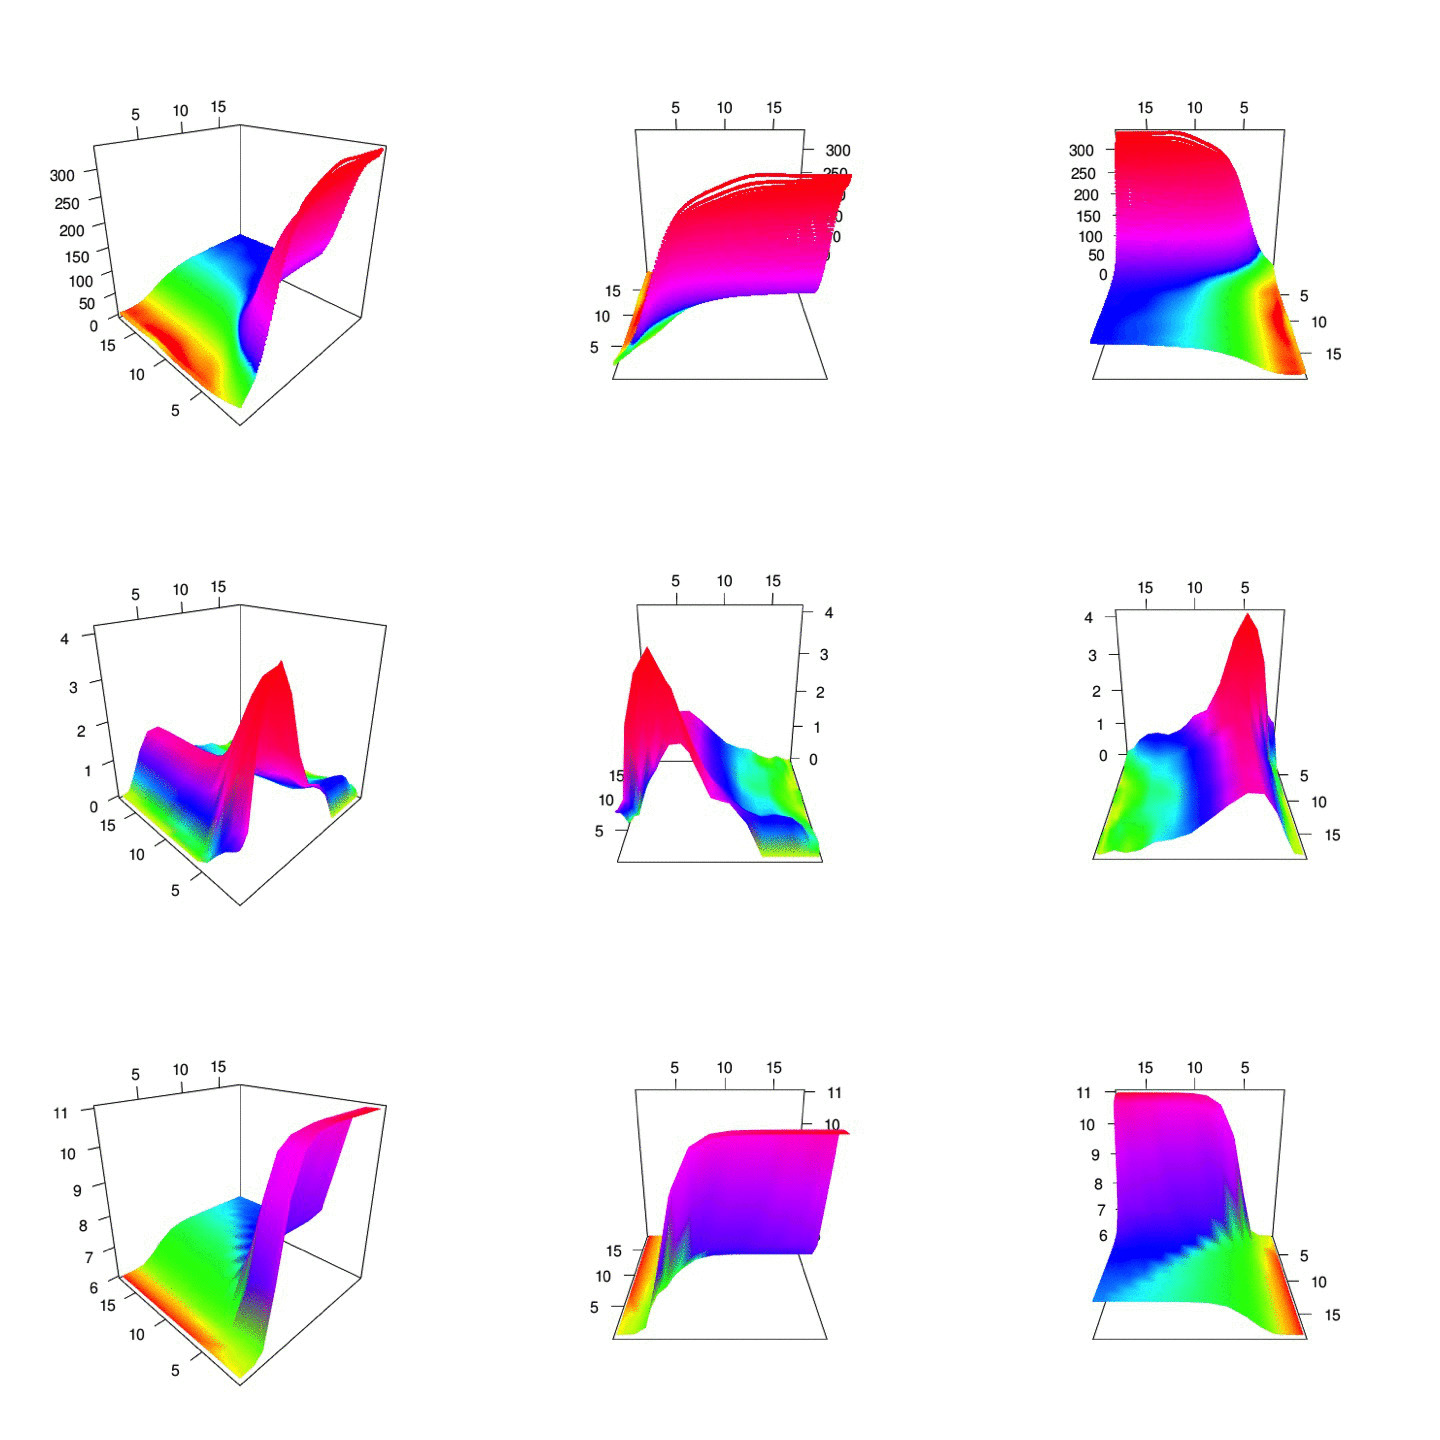
\includegraphics[width=\paperwidth]{plot_cai_18_12_eqm}}
  \caption{The equilibrium value, investment policy and pricing policy fit on an 18x18 grid with 12 degree multidimensional Chebyshev polynomials}
\end{figure}

\begin{figure}[H]
  \centering
  \makebox[\textwidth]{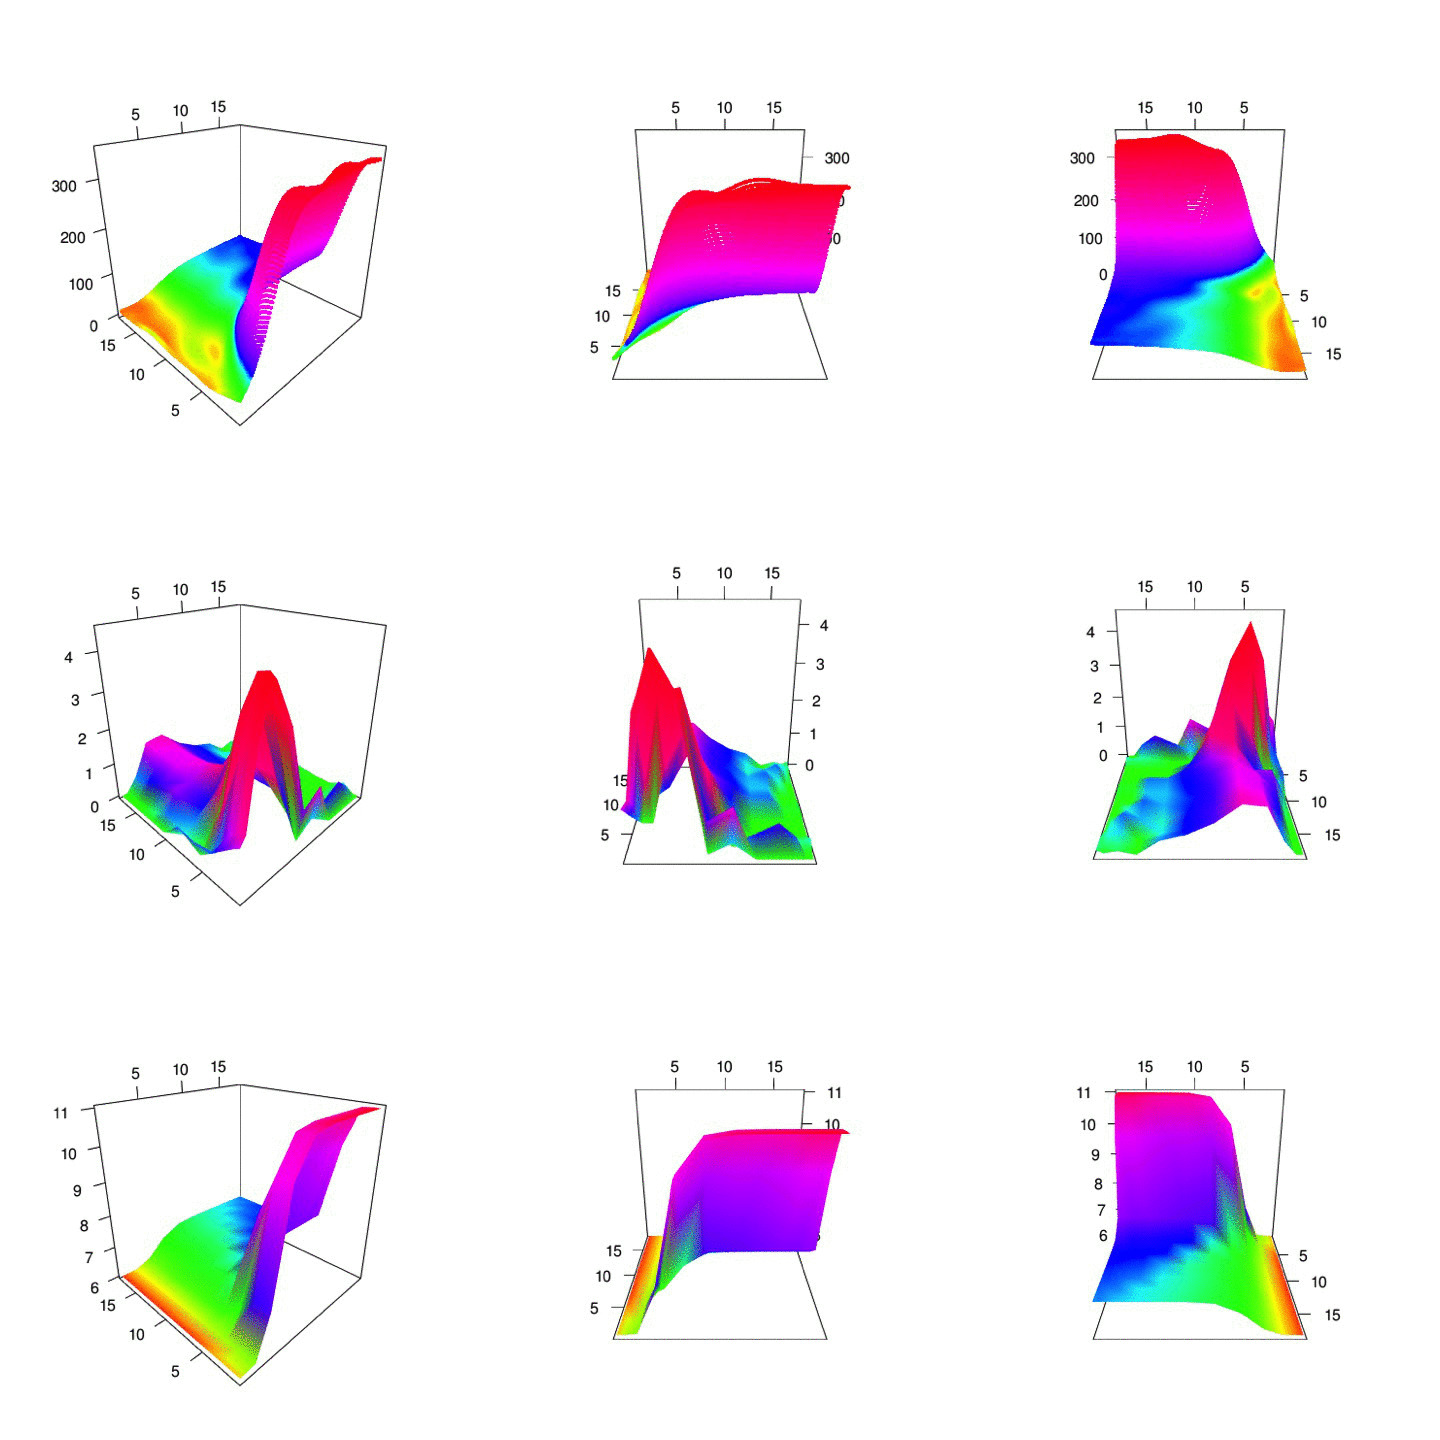
\includegraphics[width=\paperwidth]{plot_cai_12_12_eqm}}
  \caption{The equilibrium value, investment policy and pricing policy fit on an 12x12 grid with 12 degree multidimensional Chebyshev polynomials}
  \label{gibbslittle}
\end{figure}

\begin{figure}[H]
  \centering
  \makebox[\textwidth]{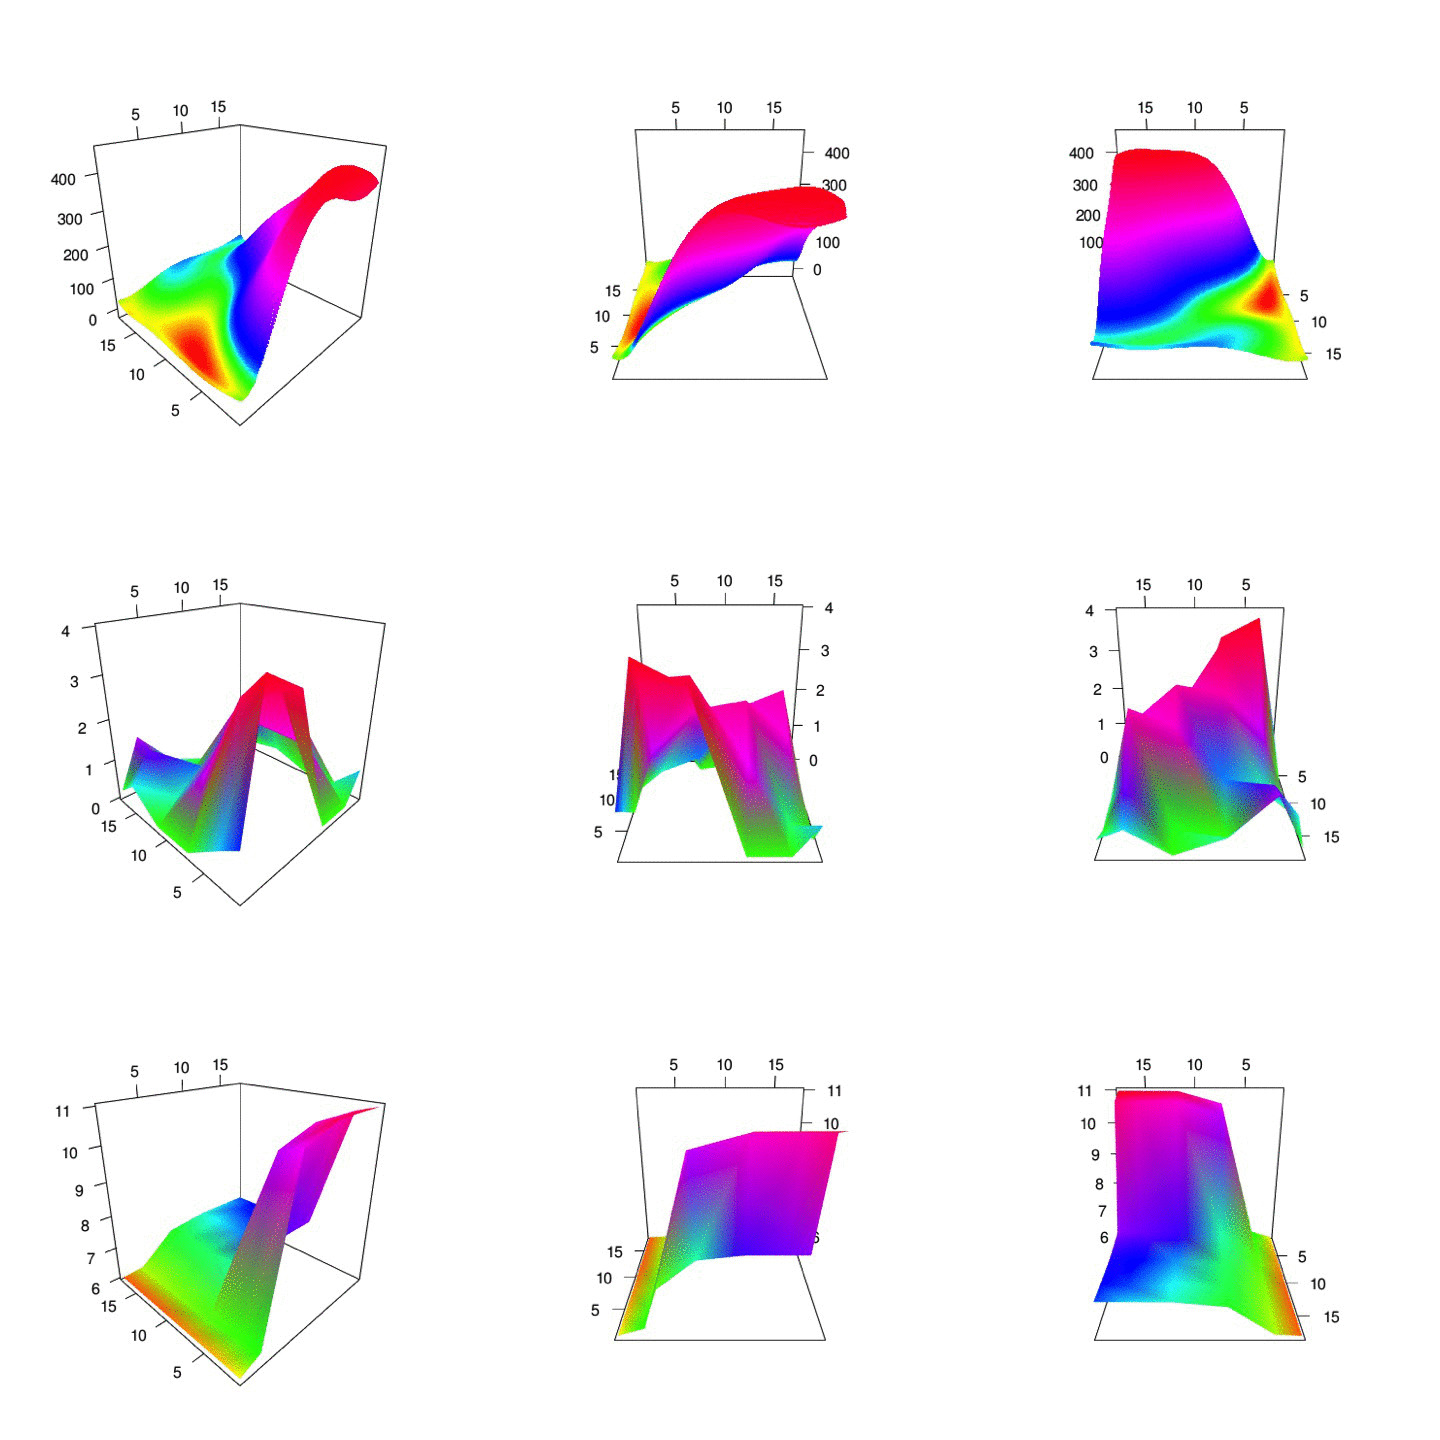
\includegraphics[width=\paperwidth]{plot_cai_6_6_eqm}}
  \caption{The equilibrium value, investment policy and pricing policy fit on an 6x6 grid with 6 degree multidimensional Chebyshev polynomials}
  \label{gibbsmore}
\end{figure}

\begin{figure}[H]
  \centering
  \makebox[\textwidth]{\includegraphics[width=\paperwidth]{plot_ann_18_eqm}}
  \caption{The equilibrium value, investment policy and pricing policy fit on an 18x18 grid using a neural net with a single fully connected layer with 324 nodes and tanh activation function}
\end{figure}

\begin{figure}[H]
  \centering
  \makebox[\textwidth]{\includegraphics[width=\paperwidth]{plot_ann_12_eqm}}
  \caption{The equilibrium value, investment policy and pricing policy fit on an 12x12 grid using a neural net with a single fully connected layer with 144 nodes and tanh activation function}
\end{figure}

\begin{figure}[H]
  \centering
  \makebox[\textwidth]{\includegraphics[width=\paperwidth]{plot_ann_6_eqm}}
  \caption{The equilibrium value, investment policy and pricing policy fit on an 6x6 grid using a neural net with a single fully connected layer with 144 nodes and tanh activation function}
\end{figure}

\section*{Appendix 2: Multidimensional complete Chebyshev polynomial approximation}
\label{multicheb}


This section is reproduced from \citet{2015_Judd_Cai} for convenience. Let the domain for the approximation be

\begin{equation*}
  \{\boldsymbol{x}=(x_1,\dots,x_d):x_{min,j}\leq x_j \leq x_{max,j}, j=1,\dots,d \},
\end{equation*}

for some real numbers $x_{min,j}$ and $x_{max,j}$ with $x_{max,j} > x_{min,j}$ for $j=1,\dots,d$. Let $\boldsymbol{x}_{min}=(x_{min,1},\dots,x_{min,d})$ and $\boldsymbol{x}_{max}=(x_{max,1},\dots,x_{max,d})$. Then we denote $[\boldsymbol{x}_{min},\boldsymbol{x}_{max}]$ as the approximation domain. Let $\alpha=(\alpha_1,\dots,\alpha_d)$ be a vector of non-negative integers. Let $T_\alpha(\boldsymbol{z})$ denote the product $\prod_{1\leq j \leq d} T_{\alpha_j}(z_j)$ for $\boldsymbol{z}=(z_1,\dots,z_d) \in [-1,1]^d$. Let
\begin{equation*}
  \boldsymbol{Z}(\boldsymbol{x})=\bigg( \frac{2x_1-x_{min,1}-x_{max,1}}{x_{max,1}-x_{min,1}},\dots,\frac{2x_1-x_{min,d}-x_{max,d}}{x_{max,d}-x_{min,d}} \bigg)
\end{equation*}

for any $\boldsymbol{x}=(x_1,\dots,x_d) \in [\boldsymbol{x}_{min},\boldsymbol{x}_{max}]$.

  Using this notation, the degree $n$ complete Chebyshev approximation for $V(\boldsymbol{x})$ is

\begin{equation*}
  \hat{V}_n(\boldsymbol{x};\boldsymbol{b})=\sum_{0 \leq |\alpha| \leq n} b_{\alpha} T_{\alpha} (\boldsymbol{Z}(\boldsymbol{x})),
\end{equation*}

where $|\alpha|=\sum_{j=1}^d \alpha_j$. The number of terms with $0\leq|\alpha|=\sum_{j=1}^d\alpha_i\leq n$ is $\binom{n+d}{d}$ for the degree $n$ complete Chebyshev approximation in $\mathbb{R}^d$.

\end{document}

%%% Local Variables:
%%% mode: latex
%%% TeX-master: t
%%% End:
